\section{Background}
\label{sec:background}

Before you start the lab, we strongly recommend you read this section. 

\subsection{Your Tools}


\subsubsection{Hardware}

You have a Raspberry Pi.
The Raspberry PI 3 Module B+ contains 4 Cortex-A53 cores, which is Armv8-A architecture.
It supports both 32-bit Armv8-A (also called aarch32) and 64-bit Armv8-A (also called aarch64) architecture.
The official kernel is compiled as 32-bit Armv8-A architecture.

\subsubsection{Boot directory}

In the SD card file system, it contains a directory, "boot", which stores the important configurations ("config.txt"), kernel ("kernel.img" or "kernel7.img"), device tree files ("*.dtb"), and etc.
In this lab, you should replace the \textbf{kernel} and necessary 
\textbf{device tree files}. 

\subsubsection{Source Code of Linux Kernel}

In the following instructions, you should download the source codes of the Linux kernel, and compile them.
You can use the prepared files, or download it from the official 
website:

\begin{lstlisting}
git clone http://github.com/raspberrypi/linux -b rpi-4.14.y
\end{lstlisting}

\subsubsection{(Cross-compile Tools}

You can compile the kernel on a virtual machine, then copy kernel image, dtb files, and modules into the disk.
However, since you want to compile a \texttt{Arm}-based kernel, and 
your virtual machine (Ubuntu) is \texttt{x86} architecture, you must 
use the \textbf{Cross Compile} tools to build the \texttt{Arm} files 
on \texttt{x86} architecture.

You can use the prepared files, or download it from the official 
website:

\begin{lstlisting}
git clone git://github.com/raspberrypi/tools.git
\end{lstlisting}




\subsection{Armv8-A Exception Levels}

In Figure~\ref{fig:armel}, Armv8-A define four exception levels (EL0 - EL3) with different privilege, and the higher number indicates the higher privilege.
The components with higher-level privileges can access the source (e.g., memory and registers) of lower-level privileges.
Detailed usage of exception levels are listed as follows:

\begin{itemize}
	\item EL0: used for user applications, such as a game.
	\item EL1: used for the kernel, including the GPU driver, virtual address management, etc.
	\item EL2: used for the hypervisor, also called as virtualization layer.
	\item EL3: used for secure monitor (not used in our defense).
\end{itemize}

\begin{figure}[htb]
	\centering
	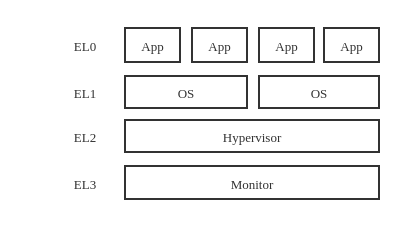
\includegraphics[width=0.6\linewidth]{el.png}
	\caption{Armv8-A Exception Level, source from
		https://developer.arm.com/documentation/den0024/a/Fundamentals-of-ARMv8}
	\label{fig:armel}
\end{figure}

In this lab, we assume the attacker controls EL0 \& EL1, and we design a defense on EL2.
Note that the EL1 attacker cannot directly access the resource in EL2 
(You can try to read an EL2 register in a kernel module, and find 
that the module is crashed). 


\begin{figure}[htb]
	\centering
	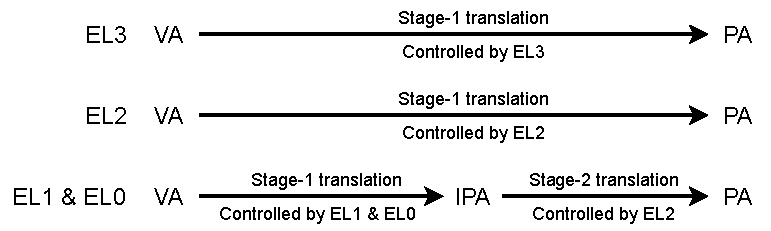
\includegraphics[width=0.8\linewidth]{s2trans_back.pdf}
	\caption{The mechanism of address translation in Armv8-A}
	\label{fig:armat}
\end{figure}

\subsection{Armv8-A Address Translation}

For memory management, Armv8-A defines 3 types of address: the virtual address (\texttt{VA}),
the intermediate physical address (\texttt{IPA}) and the physical address
(\texttt{PA}).
Armv8-A defines Stage-1 address translation for each exception level. 
Moreover, Armv8-A introduces an additional address translation for translation regime in EL0 \& EL1, called the State-2 translation, which is controlled by EL2.
As described in
Figure~\ref{fig:armat}, the VA in EL0 \& EL1 must be first translated into an IPA before reaching a PA.

If the IPA to PA is failed, the translation will not reach a correct result.
Therefore, in this lab, we can leverage the Stage-2 translation to control the access of the physical memory regions. Specifically, the region mapped to the debug registers.
